\documentclass[letterpaper]{article}
\usepackage{aaai}
\usepackage{times}
\usepackage{helvet}
\usepackage{courier}
\usepackage{graphicx}
\usepackage{amssymb}
\frenchspacing
\pdfinfo{
/Title (Hashing for Lightweight Episodic Recall)
/Subject (AAAI Publications)
/Author (Scott A. Wallace, Evan Dickinson, Andrew Nuxoll)
/Keywords(Episodic Memory,Soar,Reinforcement Learning,Hidden State)
}
\setcounter{secnumdepth}{0}  

\begin{document}
\title{Sudoku Solver}
\author{
	Benjamin Longbons\and
    Eric Klinginsmith \and 
    Sebastian S\'{a}nchez \\
Washington State University Vancouver \\
14204 NE Salmon Creek Ave. \\
Vancouver, WA 98686
}

\maketitle
\begin{abstract}
This document explores the performance of two separate implementations of sudoku puzzle agent and the resulting evaluation of the implementations. Each implementation is a distinct search method to solve any sudoku puzzle. They will be evaluated based on how fast each solves a given set of puzzles. It was our goal to explore these methods to ultimately see how well they worked.
\end{abstract}

\section{Introduction}

A sudoku puzzle like the one in Figure \ref{fig:sudoku-puzzle} is any $ n^{2} $ by $ n^{2} $ grid sub divided into $ n^{2} $, n by n boxes. In the typical case $ n $ is equal to $3$ which makes the Puzzle a $9$ by $9$ grid with $9$ boxes, each box being it's own $3$ by $3$ grid. In any case, to solve the Puzzle, distinct numbers $1$ through $ n^{2} $ must be filled into every row and column of the grid so that no two numbers are in the same row, column, or box. Our implementations solve any sudoku puzzle with an $n \not\le 7$.

\section{Implementations}

\subsection{SearchNxN Implementation}

The SearchNxN Implementation searches for the solution by filling in one box at a time. To do this, SearchNxN first selects one of the boxes to fill in. Once selected, SearchNxN will generate all possible solutions for the given box. These these solutions are added to a stack. Then for every element on the stack SearchNxN selects the next box to fill in. This process is repeated until either all boxes are filled in, or the stack is empty. If all boxes are filled in, then the solution is printed to stdout. Otherwise, there is no solution and \emph{false} is returned. The inspiration behind this method was taken from the common computer science problem of a three coloring. A three coloring is a problem in which when given a map with $n$ regions to color an agent finds a way to color the entire map with only three colors so that no two regions have the same two colors. If we think of the sudoku puzzle as being a map where no two numbers can be in the same row, column, or box and each box is a region, then a so called three coloring of a sudoku puzzle would be to "color" each box so that there are no violations where a color would be one of the possible solutions to that box.

\begin{figure}[h]
	\centering
	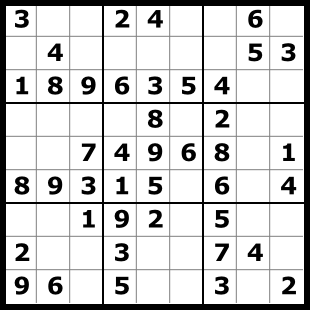
\includegraphics[width=60mm]{./Sudoku-games.png}
	\caption{Sudoku Puzzle}
	\label{fig:sudoku-puzzle}
\end{figure}

\subsection{About choosing the next box to fill in}

Before moving on we would like to explain the different ways in which SearchNxN can pick the next box to fill in. There were two methods on how to accomplish this, they are:

\begin{enumerate}
  \item inOrder
  \item mostAdjacent
\end{enumerate}

\subsubsection{inOrder}

The inOrder method of choosing the next box is the simplest method. It chooses the next box in a left to right top to bottom fashion. This method, although simple, has a very small time constraint. This makes inOrder very viable.

\subsubsection{mostAdjacent}

The mostAdjacent method of choosing the next box is a little more complicated. This function tries to reduce the branching factor of the search by choosing the next sector that will limit other sectors the most. This is accomplished by counting the number of unfilled in sectors in the same row or column of a given sector. The sector with the most unfilled in sectors in the same row or column as it is the one that this method chooses to fill in next. This idea came about because we wanted to limit the available possibilities for other surrounding boxes.

\subsection{About sole candidates}

We would like to mention one other part to our implementation. This is the idea of sole candidates. In a sudoku puzzle, there are sometimes cells were only one number can be placed there. This means that for any partially solved puzzle can have one or more sole candidates. If a sole candidate is found, then our implementation will try to find another. This continues until either all the sole candidates have been found or it hits a cell where there are no possibilities. If the result is the latter, then that branch of the search is invalid and therefore the search must then try a different path to find the solution.

\section{Experiments}
	\begin{figure}[h]
		\centering
		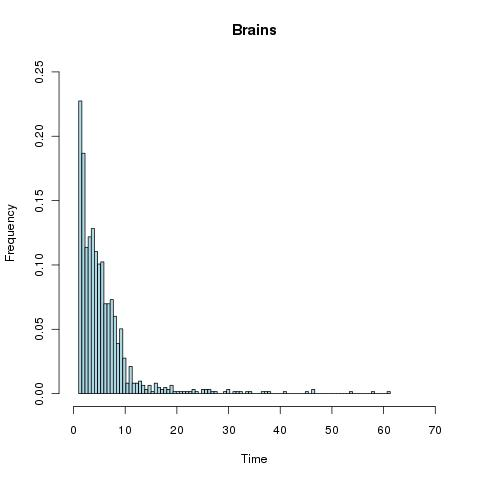
\includegraphics[width=60mm]{./brains_stats.jpg}
		\caption{Histogram for Brains Strategy}
	\label{fig:brains-strategy}
\end{figure}

\begin{tabular}{|l|l|l|l|l|l|}
\hline
Min. & 1st Qu.  & Median & Mean & 3rd Qu. & Max. \\
\hline
  1.008 & 2.212 & 4.298 & 5.844 & 7.095 & 61.290\\
\hline
\end{tabular}

\end{document}
